\documentclass[10.5pt]{article}
\def\examlang{ro}
\def\headyear{2026--2027}
% ===== Preambul comun pentru examen, banca de probleme și setul de exerciții (XeLaTeX) =====
% Serii de timp / Time Series Analysis -- Daniel Traian Pele
% Folosire: \documentclass[10.5pt]{article}  \def\examlang{ro} (sau en)  % ===== Preambul comun pentru examen, banca de probleme și setul de exerciții (XeLaTeX) =====
% Serii de timp / Time Series Analysis -- Daniel Traian Pele
% Folosire: \documentclass[10.5pt]{article}  \def\examlang{ro} (sau en)  % ===== Preambul comun pentru examen, banca de probleme și setul de exerciții (XeLaTeX) =====
% Serii de timp / Time Series Analysis -- Daniel Traian Pele
% Folosire: \documentclass[10.5pt]{article}  \def\examlang{ro} (sau en)  \input{../tsa_exam_preamble}
% Fișierele se compilează din exam/<subfolder>/, deci logo-urile sînt în ../../logos/, iar rezultatele
% software (fișiere text generate de exam/make_figs.py) se includ cu \softout{bank/out/...} sau \softout{practice/out/...}.
\usepackage{fontspec}
\setmainfont{Helvetica Neue}
\setmonofont{Menlo}[Scale=0.92]
\usepackage{amsmath,amssymb}
\usepackage[a4paper,margin=1.9cm,top=2.4cm,headsep=0.5cm,headheight=14pt]{geometry}
\usepackage{graphicx}
\usepackage{float}
\usepackage{booktabs}
\usepackage{array}
\usepackage{enumitem}
\usepackage{xcolor}
\usepackage{fancyhdr}
\usepackage{fancyvrb}
\usepackage{lastpage}
\usepackage[hidelinks]{hyperref}
\definecolor{tsablue}{RGB}{26,58,110}
\definecolor{tsared}{RGB}{205,0,0}
\graphicspath{{../../logos/}{figs/}{../bank/figs/}{../practice/figs/}}

\providecommand{\examlang}{ro}
\newif\ifen
\def\tmpen{en}\ifx\examlang\tmpen\entrue\else\enfalse\fi

% etichete
\ifen
  \renewcommand{\figurename}{Figure}\renewcommand{\tablename}{Table}
  \newcommand{\coursetitle}{Time Series Analysis}
  \newcommand{\subjword}{Problem}
  \newcommand{\rezword}{Solution.}
  \newcommand{\baremword}{Grading:}
  \newcommand{\outword}{Software output}
\else
  \renewcommand{\figurename}{Figura}\renewcommand{\tablename}{Tabelul}
  \newcommand{\coursetitle}{Serii de timp}
  \newcommand{\subjword}{Subiectul}
  \newcommand{\rezword}{Rezolvare.}
  \newcommand{\baremword}{Barem:}
  \newcommand{\outword}{Rezultatul programului}
\fi

% comutator: barem/rezolvare (true) sau subiecte (false)
\newif\ifrez \rezfalse

% antet / subsol
\pagestyle{fancy}
\fancyhf{}
\renewcommand{\headrulewidth}{0.4pt}
\lhead{\small\itshape \coursetitle}
\providecommand{\headyear}{2027}
\rhead{\small\bfseries \headyear}
\cfoot{\small\thepage/\pageref{LastPage}}

\setlength{\parindent}{0pt}
\setlength{\parskip}{0.42ex}
\setlength{\emergencystretch}{3em}

% numerotare automată, continuă, a cerințelor (1, 2, 3, ...)
\newcounter{qq}
\newcommand{\Q}{\refstepcounter{qq}\textbf{\theqq.}~}
% punctaj aliniat la dreapta, pe ultima linie a cerinței
\newcommand{\pts}[1]{\nobreak\hfill\textnormal{\itshape (#1)}\par}

% titlu de subiect: "Subiectul I • Titlu ........ puncte" + linie
\newcommand{\subiect}[3]{%
  \vspace{1.05ex}%
  {\color{tsablue}\bfseries \subjword\ #1 \textbullet\ #2}\hfill{\bfseries #3}\par
  \vspace{0.2ex}{\color{tsablue}\hrule height0.8pt}\vspace{0.7ex}}
% subiect numerotat automat (I, II, ...); argumentul opțional = identificatorul din bancă (vizibil doar în barem)
\newcounter{subj}
\newcommand{\problem}[3][]{%
  \stepcounter{subj}%
  \subiect{\Roman{subj}}{#2\ifrez\if\relax\detokenize{#1}\relax\else\ {\normalfont\footnotesize\color{tsared}[#1]}\fi\fi}{#3}}

% rezultatul unui program (statsmodels, arch, scikit-learn), inclus dintr-un fișier text generat de make_figs.py;
% calea este relativă la exam/ (de exemplu bank/out/ch02_arma.txt)
\newcommand{\softout}[1]{\par\vspace{0.3ex}%
  \VerbatimInput[fontsize=\footnotesize,frame=lines,framesep=1.2mm,rulecolor=\color{tsablue},
    label={\footnotesize\color{tsablue}\outword}]{../#1}\par\vspace{0.2ex}}

% blocul de rezolvare (doar în barem)
\newcommand{\Rez}{\par\vspace{0.2ex}\textit{\rezword}\par\nopagebreak}
\newcommand{\barem}[1]{\par\textit{\baremword\ #1}\par}

% bloc de titlu cu sigle
\newcommand{\titlublock}[1]{%
\begin{center}
  \begin{minipage}[c]{0.16\textwidth}
\includegraphics[height=1.15cm]{ase_logo.png}\end{minipage}%
  \begin{minipage}[c]{0.68\textwidth}\centering
  \ifen
    {\bfseries Bucharest University of Economic Studies}\\[0.2ex]
    Faculty of Cybernetics, Statistics and Economic Informatics\\[0.2ex]
    Course: Time Series Analysis
  \else
    {\bfseries Academia de Studii Economice din București}\\[0.2ex]
    Facultatea de Cibernetică, Statistică și Informatică Economică\\[0.2ex]
    Disciplina: Serii de timp
  \fi
  \end{minipage}%
  \begin{minipage}[c]{0.16\textwidth}\raggedleft
\includegraphics[height=0.95cm]{ida_logo.png}\end{minipage}\\[1.2ex]
  {\large\bfseries #1}
\end{center}}

% valori utile generale (z_p, chi^2_p = cuantile de ordin p; valori critice Dickey--Fuller pentru eșantioane mari)
\newcommand{\valoriutilegen}{%
\ifen Useful values: $z_{0.975}=1.960$, $z_{0.95}=1.645$, $\chi^2_{0.95}(1)=3.84$, $\chi^2_{0.95}(2)=5.99$,
$\chi^2_{0.95}(3)=7.81$, $\chi^2_{0.95}(4)=9.49$, $\chi^2_{0.95}(5)=11.07$, $\chi^2_{0.95}(6)=12.59$,
$\chi^2_{0.95}(8)=15.51$, $\chi^2_{0.95}(10)=18.31$, $\chi^2_{0.95}(12)=21.03$, $\chi^2_{0.95}(20)=31.41$;
5\% Dickey--Fuller critical values: $-1.95$ (no constant), $-2.86$ (constant), $-3.41$ (constant and trend);
$\ln 2=0.693$ ($z_p$ and $\chi^2_p$ are quantiles of order $p$).
\else Valori utile: $z_{0,975}=1{,}960$; $z_{0,95}=1{,}645$; $\chi^2_{0,95}(1)=3{,}84$; $\chi^2_{0,95}(2)=5{,}99$;
$\chi^2_{0,95}(3)=7{,}81$; $\chi^2_{0,95}(4)=9{,}49$; $\chi^2_{0,95}(5)=11{,}07$; $\chi^2_{0,95}(6)=12{,}59$;
$\chi^2_{0,95}(8)=15{,}51$; $\chi^2_{0,95}(10)=18{,}31$; $\chi^2_{0,95}(12)=21{,}03$; $\chi^2_{0,95}(20)=31{,}41$;
valorile critice Dickey--Fuller la 5\%: $-1{,}95$ (fără constantă); $-2{,}86$ (cu constantă); $-3{,}41$ (constantă
și trend); $\ln 2=0{,}693$ ($z_p$ și $\chi^2_p$ sînt cuantile de ordin $p$).\fi}

% titlul capitolului într-un fișier din bancă (folosit doar ca etichetă de build_variant.py)
\newcommand{\banktitle}[2]{}

% Fișierele se compilează din exam/<subfolder>/, deci logo-urile sînt în ../../logos/, iar rezultatele
% software (fișiere text generate de exam/make_figs.py) se includ cu \softout{bank/out/...} sau \softout{practice/out/...}.
\usepackage{fontspec}
\setmainfont{Helvetica Neue}
\setmonofont{Menlo}[Scale=0.92]
\usepackage{amsmath,amssymb}
\usepackage[a4paper,margin=1.9cm,top=2.4cm,headsep=0.5cm,headheight=14pt]{geometry}
\usepackage{graphicx}
\usepackage{float}
\usepackage{booktabs}
\usepackage{array}
\usepackage{enumitem}
\usepackage{xcolor}
\usepackage{fancyhdr}
\usepackage{fancyvrb}
\usepackage{lastpage}
\usepackage[hidelinks]{hyperref}
\definecolor{tsablue}{RGB}{26,58,110}
\definecolor{tsared}{RGB}{205,0,0}
\graphicspath{{../../logos/}{figs/}{../bank/figs/}{../practice/figs/}}

\providecommand{\examlang}{ro}
\newif\ifen
\def\tmpen{en}\ifx\examlang\tmpen\entrue\else\enfalse\fi

% etichete
\ifen
  \renewcommand{\figurename}{Figure}\renewcommand{\tablename}{Table}
  \newcommand{\coursetitle}{Time Series Analysis}
  \newcommand{\subjword}{Problem}
  \newcommand{\rezword}{Solution.}
  \newcommand{\baremword}{Grading:}
  \newcommand{\outword}{Software output}
\else
  \renewcommand{\figurename}{Figura}\renewcommand{\tablename}{Tabelul}
  \newcommand{\coursetitle}{Serii de timp}
  \newcommand{\subjword}{Subiectul}
  \newcommand{\rezword}{Rezolvare.}
  \newcommand{\baremword}{Barem:}
  \newcommand{\outword}{Rezultatul programului}
\fi

% comutator: barem/rezolvare (true) sau subiecte (false)
\newif\ifrez \rezfalse

% antet / subsol
\pagestyle{fancy}
\fancyhf{}
\renewcommand{\headrulewidth}{0.4pt}
\lhead{\small\itshape \coursetitle}
\providecommand{\headyear}{2027}
\rhead{\small\bfseries \headyear}
\cfoot{\small\thepage/\pageref{LastPage}}

\setlength{\parindent}{0pt}
\setlength{\parskip}{0.42ex}
\setlength{\emergencystretch}{3em}

% numerotare automată, continuă, a cerințelor (1, 2, 3, ...)
\newcounter{qq}
\newcommand{\Q}{\refstepcounter{qq}\textbf{\theqq.}~}
% punctaj aliniat la dreapta, pe ultima linie a cerinței
\newcommand{\pts}[1]{\nobreak\hfill\textnormal{\itshape (#1)}\par}

% titlu de subiect: "Subiectul I • Titlu ........ puncte" + linie
\newcommand{\subiect}[3]{%
  \vspace{1.05ex}%
  {\color{tsablue}\bfseries \subjword\ #1 \textbullet\ #2}\hfill{\bfseries #3}\par
  \vspace{0.2ex}{\color{tsablue}\hrule height0.8pt}\vspace{0.7ex}}
% subiect numerotat automat (I, II, ...); argumentul opțional = identificatorul din bancă (vizibil doar în barem)
\newcounter{subj}
\newcommand{\problem}[3][]{%
  \stepcounter{subj}%
  \subiect{\Roman{subj}}{#2\ifrez\if\relax\detokenize{#1}\relax\else\ {\normalfont\footnotesize\color{tsared}[#1]}\fi\fi}{#3}}

% rezultatul unui program (statsmodels, arch, scikit-learn), inclus dintr-un fișier text generat de make_figs.py;
% calea este relativă la exam/ (de exemplu bank/out/ch02_arma.txt)
\newcommand{\softout}[1]{\par\vspace{0.3ex}%
  \VerbatimInput[fontsize=\footnotesize,frame=lines,framesep=1.2mm,rulecolor=\color{tsablue},
    label={\footnotesize\color{tsablue}\outword}]{../#1}\par\vspace{0.2ex}}

% blocul de rezolvare (doar în barem)
\newcommand{\Rez}{\par\vspace{0.2ex}\textit{\rezword}\par\nopagebreak}
\newcommand{\barem}[1]{\par\textit{\baremword\ #1}\par}

% bloc de titlu cu sigle
\newcommand{\titlublock}[1]{%
\begin{center}
  \begin{minipage}[c]{0.16\textwidth}
\includegraphics[height=1.15cm]{ase_logo.png}\end{minipage}%
  \begin{minipage}[c]{0.68\textwidth}\centering
  \ifen
    {\bfseries Bucharest University of Economic Studies}\\[0.2ex]
    Faculty of Cybernetics, Statistics and Economic Informatics\\[0.2ex]
    Course: Time Series Analysis
  \else
    {\bfseries Academia de Studii Economice din București}\\[0.2ex]
    Facultatea de Cibernetică, Statistică și Informatică Economică\\[0.2ex]
    Disciplina: Serii de timp
  \fi
  \end{minipage}%
  \begin{minipage}[c]{0.16\textwidth}\raggedleft
\includegraphics[height=0.95cm]{ida_logo.png}\end{minipage}\\[1.2ex]
  {\large\bfseries #1}
\end{center}}

% valori utile generale (z_p, chi^2_p = cuantile de ordin p; valori critice Dickey--Fuller pentru eșantioane mari)
\newcommand{\valoriutilegen}{%
\ifen Useful values: $z_{0.975}=1.960$, $z_{0.95}=1.645$, $\chi^2_{0.95}(1)=3.84$, $\chi^2_{0.95}(2)=5.99$,
$\chi^2_{0.95}(3)=7.81$, $\chi^2_{0.95}(4)=9.49$, $\chi^2_{0.95}(5)=11.07$, $\chi^2_{0.95}(6)=12.59$,
$\chi^2_{0.95}(8)=15.51$, $\chi^2_{0.95}(10)=18.31$, $\chi^2_{0.95}(12)=21.03$, $\chi^2_{0.95}(20)=31.41$;
5\% Dickey--Fuller critical values: $-1.95$ (no constant), $-2.86$ (constant), $-3.41$ (constant and trend);
$\ln 2=0.693$ ($z_p$ and $\chi^2_p$ are quantiles of order $p$).
\else Valori utile: $z_{0,975}=1{,}960$; $z_{0,95}=1{,}645$; $\chi^2_{0,95}(1)=3{,}84$; $\chi^2_{0,95}(2)=5{,}99$;
$\chi^2_{0,95}(3)=7{,}81$; $\chi^2_{0,95}(4)=9{,}49$; $\chi^2_{0,95}(5)=11{,}07$; $\chi^2_{0,95}(6)=12{,}59$;
$\chi^2_{0,95}(8)=15{,}51$; $\chi^2_{0,95}(10)=18{,}31$; $\chi^2_{0,95}(12)=21{,}03$; $\chi^2_{0,95}(20)=31{,}41$;
valorile critice Dickey--Fuller la 5\%: $-1{,}95$ (fără constantă); $-2{,}86$ (cu constantă); $-3{,}41$ (constantă
și trend); $\ln 2=0{,}693$ ($z_p$ și $\chi^2_p$ sînt cuantile de ordin $p$).\fi}

% titlul capitolului într-un fișier din bancă (folosit doar ca etichetă de build_variant.py)
\newcommand{\banktitle}[2]{}

% Fișierele se compilează din exam/<subfolder>/, deci logo-urile sînt în ../../logos/, iar rezultatele
% software (fișiere text generate de exam/make_figs.py) se includ cu \softout{bank/out/...} sau \softout{practice/out/...}.
\usepackage{fontspec}
\setmainfont{Helvetica Neue}
\setmonofont{Menlo}[Scale=0.92]
\usepackage{amsmath,amssymb}
\usepackage[a4paper,margin=1.9cm,top=2.4cm,headsep=0.5cm,headheight=14pt]{geometry}
\usepackage{graphicx}
\usepackage{float}
\usepackage{booktabs}
\usepackage{array}
\usepackage{enumitem}
\usepackage{xcolor}
\usepackage{fancyhdr}
\usepackage{fancyvrb}
\usepackage{lastpage}
\usepackage[hidelinks]{hyperref}
\definecolor{tsablue}{RGB}{26,58,110}
\definecolor{tsared}{RGB}{205,0,0}
\graphicspath{{../../logos/}{figs/}{../bank/figs/}{../practice/figs/}}

\providecommand{\examlang}{ro}
\newif\ifen
\def\tmpen{en}\ifx\examlang\tmpen\entrue\else\enfalse\fi

% etichete
\ifen
  \renewcommand{\figurename}{Figure}\renewcommand{\tablename}{Table}
  \newcommand{\coursetitle}{Time Series Analysis}
  \newcommand{\subjword}{Problem}
  \newcommand{\rezword}{Solution.}
  \newcommand{\baremword}{Grading:}
  \newcommand{\outword}{Software output}
\else
  \renewcommand{\figurename}{Figura}\renewcommand{\tablename}{Tabelul}
  \newcommand{\coursetitle}{Serii de timp}
  \newcommand{\subjword}{Subiectul}
  \newcommand{\rezword}{Rezolvare.}
  \newcommand{\baremword}{Barem:}
  \newcommand{\outword}{Rezultatul programului}
\fi

% comutator: barem/rezolvare (true) sau subiecte (false)
\newif\ifrez \rezfalse

% antet / subsol
\pagestyle{fancy}
\fancyhf{}
\renewcommand{\headrulewidth}{0.4pt}
\lhead{\small\itshape \coursetitle}
\providecommand{\headyear}{2027}
\rhead{\small\bfseries \headyear}
\cfoot{\small\thepage/\pageref{LastPage}}

\setlength{\parindent}{0pt}
\setlength{\parskip}{0.42ex}
\setlength{\emergencystretch}{3em}

% numerotare automată, continuă, a cerințelor (1, 2, 3, ...)
\newcounter{qq}
\newcommand{\Q}{\refstepcounter{qq}\textbf{\theqq.}~}
% punctaj aliniat la dreapta, pe ultima linie a cerinței
\newcommand{\pts}[1]{\nobreak\hfill\textnormal{\itshape (#1)}\par}

% titlu de subiect: "Subiectul I • Titlu ........ puncte" + linie
\newcommand{\subiect}[3]{%
  \vspace{1.05ex}%
  {\color{tsablue}\bfseries \subjword\ #1 \textbullet\ #2}\hfill{\bfseries #3}\par
  \vspace{0.2ex}{\color{tsablue}\hrule height0.8pt}\vspace{0.7ex}}
% subiect numerotat automat (I, II, ...); argumentul opțional = identificatorul din bancă (vizibil doar în barem)
\newcounter{subj}
\newcommand{\problem}[3][]{%
  \stepcounter{subj}%
  \subiect{\Roman{subj}}{#2\ifrez\if\relax\detokenize{#1}\relax\else\ {\normalfont\footnotesize\color{tsared}[#1]}\fi\fi}{#3}}

% rezultatul unui program (statsmodels, arch, scikit-learn), inclus dintr-un fișier text generat de make_figs.py;
% calea este relativă la exam/ (de exemplu bank/out/ch02_arma.txt)
\newcommand{\softout}[1]{\par\vspace{0.3ex}%
  \VerbatimInput[fontsize=\footnotesize,frame=lines,framesep=1.2mm,rulecolor=\color{tsablue},
    label={\footnotesize\color{tsablue}\outword}]{../#1}\par\vspace{0.2ex}}

% blocul de rezolvare (doar în barem)
\newcommand{\Rez}{\par\vspace{0.2ex}\textit{\rezword}\par\nopagebreak}
\newcommand{\barem}[1]{\par\textit{\baremword\ #1}\par}

% bloc de titlu cu sigle
\newcommand{\titlublock}[1]{%
\begin{center}
  \begin{minipage}[c]{0.16\textwidth}
\includegraphics[height=1.15cm]{ase_logo.png}\end{minipage}%
  \begin{minipage}[c]{0.68\textwidth}\centering
  \ifen
    {\bfseries Bucharest University of Economic Studies}\\[0.2ex]
    Faculty of Cybernetics, Statistics and Economic Informatics\\[0.2ex]
    Course: Time Series Analysis
  \else
    {\bfseries Academia de Studii Economice din București}\\[0.2ex]
    Facultatea de Cibernetică, Statistică și Informatică Economică\\[0.2ex]
    Disciplina: Serii de timp
  \fi
  \end{minipage}%
  \begin{minipage}[c]{0.16\textwidth}\raggedleft
\includegraphics[height=0.95cm]{ida_logo.png}\end{minipage}\\[1.2ex]
  {\large\bfseries #1}
\end{center}}

% valori utile generale (z_p, chi^2_p = cuantile de ordin p; valori critice Dickey--Fuller pentru eșantioane mari)
\newcommand{\valoriutilegen}{%
\ifen Useful values: $z_{0.975}=1.960$, $z_{0.95}=1.645$, $\chi^2_{0.95}(1)=3.84$, $\chi^2_{0.95}(2)=5.99$,
$\chi^2_{0.95}(3)=7.81$, $\chi^2_{0.95}(4)=9.49$, $\chi^2_{0.95}(5)=11.07$, $\chi^2_{0.95}(6)=12.59$,
$\chi^2_{0.95}(8)=15.51$, $\chi^2_{0.95}(10)=18.31$, $\chi^2_{0.95}(12)=21.03$, $\chi^2_{0.95}(20)=31.41$;
5\% Dickey--Fuller critical values: $-1.95$ (no constant), $-2.86$ (constant), $-3.41$ (constant and trend);
$\ln 2=0.693$ ($z_p$ and $\chi^2_p$ are quantiles of order $p$).
\else Valori utile: $z_{0,975}=1{,}960$; $z_{0,95}=1{,}645$; $\chi^2_{0,95}(1)=3{,}84$; $\chi^2_{0,95}(2)=5{,}99$;
$\chi^2_{0,95}(3)=7{,}81$; $\chi^2_{0,95}(4)=9{,}49$; $\chi^2_{0,95}(5)=11{,}07$; $\chi^2_{0,95}(6)=12{,}59$;
$\chi^2_{0,95}(8)=15{,}51$; $\chi^2_{0,95}(10)=18{,}31$; $\chi^2_{0,95}(12)=21{,}03$; $\chi^2_{0,95}(20)=31{,}41$;
valorile critice Dickey--Fuller la 5\%: $-1{,}95$ (fără constantă); $-2{,}86$ (cu constantă); $-3{,}41$ (constantă
și trend); $\ln 2=0{,}693$ ($z_p$ și $\chi^2_p$ sînt cuantile de ordin $p$).\fi}

% titlul capitolului într-un fișier din bancă (folosit doar ca etichetă de build_variant.py)
\newcommand{\banktitle}[2]{}

\renewcommand{\subjword}{Problema}
\newcommand{\pp}[1]{\stepcounter{subj}\subiect{\arabic{subj}}{#1}{}}
\newcommand{\capitol}[1]{\par\vspace{1.4ex}{\large\bfseries\color{tsared}#1}\par\vspace{0.4ex}}
\setlist[enumerate]{label=(\alph*),leftmargin=2.2em,itemsep=0.15ex,topsep=0.3ex}
\begin{document}
\titlublock{PROBLEME DE EXAMEN --- SET DE EXERCIȚII}

\noindent Problemele au forma subiectelor de examen: interpretarea rezultatului unui program, o derivare scurtă sau
alegerea unui model. Datele provin din seriile folosite la curs (ultima zi: 18 septembrie 2026), iar rezultatele
programelor (\texttt{statsmodels}, \texttt{arch}, \texttt{scikit-learn}) sînt afișate în formatul programului, cu punct
zecimal. Răspunsurile numerice sînt la sfîrșitul documentului.
Notații: $\varepsilon_t$ zgomot alb cu varianța $\sigma^2$; $L$ operatorul lag; $r_t=100\ln(P_t/P_{t-1})$ randamentul
logaritmic în \%; $\mathrm{VaR}_\alpha=-q_\alpha$ (VaR 1\% este pierderea depășită în 1\% din zile).\par
\vspace{0.4ex}{\small\noindent\valoriutilegen\par}

% ===================================================================================================
\capitol{Capitolul 1. Procese stochastice și staționaritate}

\pp{Corelograma debitului Nilului}
Debitul anual al Nilului la Aswan ($10^8$ m$^3$, 1871--1970, $n=100$, media $919{,}4$) are corelograma de mai jos.
\softout{practice/out/p_nile_corr.txt}
\begin{enumerate}
\item Calculați limitele benzii de încredere de 95\% pentru autocorelațiile de selecție, în ipoteza de zgomot alb.
\item Formulați decizia testului Ljung--Box cu 10 decalaje, la nivelul de semnificație de 5\%.
\item Indicați modelul ARMA sugerat de tiparul funcțiilor ACF și PACF.
\end{enumerate}

\pp{Randamentul obligațiunilor SUA la 10 ani: nivel și variație}
Figura~\ref{fig:us10y} arată randamentul titlurilor de stat americane la 10 ani (zilnic, 2015--2026) și variația lui
zilnică, în puncte de bază. Pentru nivel, primele cinci autocorelații de selecție sînt $0{,}998$; $0{,}997$; $0{,}995$;
$0{,}993$; $0{,}992$. Pentru variația zilnică ($n=2926$) ele sînt $-0{,}037$; $-0{,}036$; $0{,}006$; $-0{,}012$;
$-0{,}008$.
\begin{figure}[H]\centering
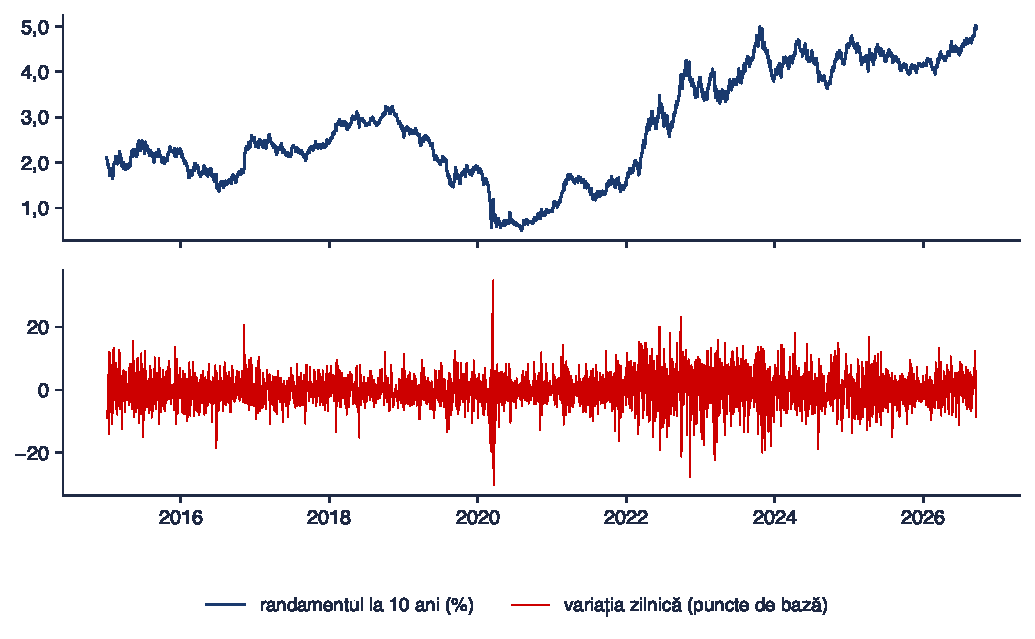
\includegraphics[width=0.66\textwidth]{practice_us10y_ro.pdf}
\caption{Randamentul la 10 ani al titlurilor de stat ale SUA și variația lui zilnică, 2015--2026.}\label{fig:us10y}
\end{figure}
\begin{enumerate}
\item Calculați statistica Ljung--Box $Q(5)=n(n+2)\sum_{k=1}^{5}\hat\rho_k^2/(n-k)$ pentru variația zilnică.
\item Formulați decizia testului la nivelul de semnificație de 5\%.
\item Explicați de ce autocorelațiile apropiate de 1 ale nivelului nu indică o serie staționară.
\end{enumerate}

\pp{Un zgomot alb care nu este independent}
Fie $Y_t=\varepsilon_t\varepsilon_{t-1}$, unde $\varepsilon_t$ sînt variabile independente $N(0,\sigma^2)$, deci
$E(\varepsilon_t^4)=3\sigma^4$.
\begin{enumerate}
\item Calculați media și varianța lui $Y_t$.
\item Arătați că $\mathrm{Cov}(Y_t,Y_{t-k})=0$ pentru orice $k\ge 1$.
\item Calculați corelația dintre $Y_t^2$ și $Y_{t-1}^2$.
\end{enumerate}

% ===================================================================================================
\capitol{Capitolul 2. Modele ARMA}

\pp{Modelul AR(2) al petelor solare}
Numărul anual de pete solare (1700--2008) a fost modelat cu un AR(2) cu constantă,
$y_t-\mu=\phi_1(y_{t-1}-\mu)+\phi_2(y_{t-2}-\mu)+\varepsilon_t$ (în \texttt{statsmodels}, \texttt{const} este media $\mu$).
\softout{practice/out/p_sunspots_ar2.txt}
Valorile observate sînt $y_{2007}=7{,}5$ și $y_{2008}=2{,}9$.
\begin{enumerate}
\item Verificați condițiile de staționaritate ale modelului AR(2) estimat.
\item Arătați că rădăcinile polinomului autoregresiv sînt complexe.
\item Calculați perioada ciclului din relația $\cos(2\pi/P)=\phi_1/\bigl(2\sqrt{-\phi_2}\bigr)$.
\item Calculați prognoza pentru 2009.
\end{enumerate}

\pp{Alegerea ordinului ARMA: producția industrială a SUA}
Pentru creșterea lunară a producției industriale a SUA, $g_t=100\,\Delta\ln \mathrm{INDPRO}_t$, s-au estimat șase
modele ARMA cu constantă.
\softout{practice/out/p_indpro_orders.txt}
Modelul AR(1) estimat este $g_t=0{,}116+0{,}202\,(g_{t-1}-0{,}116)+\varepsilon_t$, cu $\hat\sigma^2=1{,}015$; în
decembrie 2025, $g_T=0{,}454$.
\begin{enumerate}
\item Precizați modelul ales de AIC și modelul ales de BIC.
\item Interpretați coloana cu valorile $p$ ale testului Ljung--Box aplicat reziduurilor.
\item Calculați prognozele modelului AR(1) pentru ianuarie și februarie 2026.
\item Calculați abaterea standard a erorii de prognoză pe doi pași.
\end{enumerate}

\pp{Autocorelația unui MA(1)}
Fie $y_t=\varepsilon_t+\theta\varepsilon_{t-1}$.
\begin{enumerate}
\item Arătați că $\rho(1)=\theta/(1+\theta^2)$ și $\rho(k)=0$ pentru $k\ge 2$.
\item Determinați valorile lui $\theta$ pentru care $\rho(1)=0{,}4$.
\item Justificați alegerea uneia dintre cele două valori.
\end{enumerate}

% ===================================================================================================
\capitol{Capitolul 3. Rădăcini unitare și modele ARIMA}

\pp{Testul ADF pentru prețul aurului}
Pentru logaritmul prețului lunar al aurului (USD pe uncie, ianuarie 2010 -- august 2026) s-a aplicat testul
Dickey--Fuller augmentat (ADF), pe nivel și pe prima diferență.
\softout{practice/out/p_gold_adf.txt}
\begin{enumerate}
\item Formulați decizia testului pentru nivel, la nivelul de semnificație de 5\%.
\item Formulați decizia testului pentru prima diferență.
\item Precizați ordinul de integrare al seriei.
\item Explicați alegerea termenilor determiniști în cele două regresii.
\end{enumerate}

\pp{Prognoza ARIMA(0,1,1) cu derivă: aurul}
Pentru $y_t=100\ln P_t$ (prețul lunar al aurului) s-a estimat modelul $\Delta y_t=c+\varepsilon_t+\theta\varepsilon_{t-1}$.
\softout{practice/out/p_gold_ima.txt}
\begin{enumerate}
\item Testați semnificația coeficientului $\theta$.
\item Precizați modelul mai simplu sugerat de rezultat.
\item Calculați prognozele pentru septembrie și octombrie 2026, cu modelul estimat.
\item Calculați abaterile standard ale erorilor de prognoză pe unu și pe doi pași, știind că
$\psi_1=1+\theta$.
\item Transformați prognoza pentru septembrie 2026 în preț (USD pe uncie).
\end{enumerate}

\pp{ADF și KPSS pentru prețurile de consum din SUA}
Pentru indicele prețurilor de consum din SUA (CPIAUCSL, lunar, 1990--2025) s-au aplicat testele ADF (ipoteza nulă:
rădăcină unitară) și KPSS (ipoteza nulă: staționaritate).
\softout{practice/out/p_cpi_tests.txt}
\begin{enumerate}
\item Formulați concluzia comună a celor două teste pentru $\ln \mathrm{CPI}$.
\item Formulați concluzia comună pentru rata inflației.
\item Precizați ordinul de integrare al lui $\ln \mathrm{CPI}$.
\end{enumerate}

% ===================================================================================================
\capitol{Capitolul 4. Sezonalitate și prognoză}

\pp{Modelul airline pentru concentrația de CO$_2$}
Concentrația lunară de CO$_2$ la Mauna Loa (ppm, 1960--2000) a fost modelată cu un SARIMA$(0,1,1)(0,1,1)_{12}$.
\softout{practice/out/p_co2_airline.txt}
\begin{enumerate}
\item Scrieți ecuația modelului cu operatorul lag.
\item Calculați coeficientul lui $\varepsilon_{t-13}$.
\item Formulați decizia testului Ljung--Box pentru reziduuri ($24-2=22$ de grade de libertate;
$\chi^2_{0{,}95}(22)=33{,}92$).
\item Calculați autocorelațiile teoretice $\rho(1)$ și $\rho(12)$ ale seriei $(1-L)(1-L^{12})y_t$.
\end{enumerate}

\pp{Evaluarea prognozelor: înnoptările turistice din România}
Pentru numărul lunar de înnoptări în unitățile de cazare turistică din România (milioane, Eurostat), anul 2025 a fost
prognozat din decembrie 2024 cu metoda naivă sezonieră și cu un model SARIMA (Figura~\ref{fig:tour}).
\softout{practice/out/p_tourism_eval.txt}
Pentru diferențele $d_t=|e_t^{\text{naivă}}|-|e_t^{\text{SARIMA}}|$ ale celor 12 luni, media este $\bar d=-0{,}1234$, iar
abaterea standard este $s_d=0{,}210$.
\begin{figure}[H]\centering
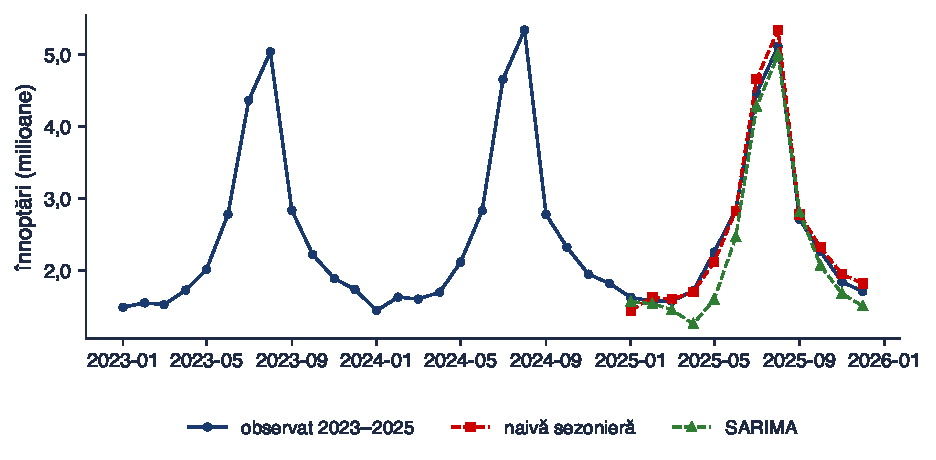
\includegraphics[width=0.66\textwidth]{practice_tourism_ro.pdf}
\caption{Înnoptări lunare în România și prognozele pentru 2025.}\label{fig:tour}
\end{figure}
\begin{enumerate}
\item Calculați MASE pentru cele două metode.
\item Calculați statistica Diebold--Mariano $\mathrm{DM}=\bar d/(s_d/\sqrt{12})$.
\item Formulați decizia testului Diebold--Mariano la nivelul de semnificație de 5\%.
\item Explicați rezultatul slab al modelului SARIMA.
\end{enumerate}

\pp{Diferența sezonieră}
În iulie și august 2024, înnoptările au fost $4{,}660$ și $5{,}346$ milioane, iar în iulie și august 2025, $4{,}467$ și
$5{,}117$ milioane.
\begin{enumerate}
\item Calculați $\Delta_{12}\ln y_t=\ln y_t-\ln y_{t-12}$ pentru iulie și august 2025, în \%.
\item Arătați că $1-L^{12}=(1-L)(1+L+\dots+L^{11})$.
\item Arătați că $\Delta_{12}$ elimină o componentă sezonieră deterministă $s_t=s_{t-12}$.
\end{enumerate}

% ===================================================================================================
\capitol{Capitolul 5. Volatilitate condiționată și modele GARCH}

\pp{GARCH(1,1)-$t$ pentru DAX}
Pentru randamentele logaritmice zilnice ale indicelui DAX s-a estimat modelul
$\sigma_t^2=\omega+\alpha\varepsilon_{t-1}^2+\beta\sigma_{t-1}^2$, cu inovații Student-$t$.
\softout{practice/out/p_dax_garch.txt}
\begin{enumerate}
\item Calculați persistența volatilității.
\item Calculați volatilitatea de lungă durată, zilnică și anualizată (252 de zile).
\item Calculați timpul de înjumătățire al unui șoc de volatilitate.
\item Calculați excesul de boltire al inovațiilor Student-$t$, $6/(\nu-4)$.
\item Interpretați excesul de boltire al inovațiilor.
\end{enumerate}

\pp{Un pas GARCH și VaR 1\%: Ethereum}
Un GARCH(1,1) cu inovații Normale, estimat pe randamentele zilnice ale Ethereum (2018--2026), are
$\hat\mu=0{,}083$; $\hat\omega=0{,}503$; $\hat\alpha=0{,}064$; $\hat\beta=0{,}911$. Pe 18 septembrie 2026, varianța
condiționată a fost $\sigma_T^2=10{,}225$, iar randamentul a fost $r_T=6{,}496\%$. Se dă $z_{0{,}01}=-2{,}326$.
\begin{enumerate}
\item Calculați varianța condiționată pentru 19 septembrie 2026.
\item Calculați VaR 1\% pentru 19 septembrie 2026, în \%.
\item Calculați pierderea corespunzătoare pentru o poziție de 10\,000 USD.
\end{enumerate}

\pp{Asimetria volatilității: GJR-GARCH pentru DAX}
Pe aceleași date DAX s-a estimat un GJR-GARCH(1,1,1) cu inovații Student-$t$,
$\sigma_t^2=\omega+(\alpha+\gamma I_{t-1})\varepsilon_{t-1}^2+\beta\sigma_{t-1}^2$, unde $I_{t-1}=1$ dacă
$\varepsilon_{t-1}<0$.
\softout{practice/out/p_dax_gjr.txt}
\begin{enumerate}
\item Testați modelul GARCH(1,1)-$t$ față de GJR-GARCH cu un test al raportului de verosimilitate.
\item Calculați $\sigma_t^2$ după un șoc $\varepsilon_{t-1}=-2$ și după un șoc $\varepsilon_{t-1}=+2$, cu $\sigma_{t-1}^2=1$.
\item Calculați persistența $\alpha+\gamma/2+\beta$.
\item Interpretați estimarea $\hat\alpha=0$.
\end{enumerate}

% ===================================================================================================
\capitol{Capitolul 6. Modele VAR și cauzalitate Granger}

\pp{Un VAR macroeconomic: SUA, 1959--2009}
Pentru vectorul format din creșterea PIB-ului real (anualizată, \%), inflație și rata dobînzii la titlurile de stat pe
3 luni (date trimestriale, setul \texttt{macrodata}) s-au calculat criteriile informaționale și testele de cauzalitate
Granger într-un VAR(2) cu constantă.
\softout{practice/out/p_macro_var.txt}
\begin{enumerate}
\item Precizați ordinul ales de fiecare criteriu informațional.
\item Calculați numărul de coeficienți ai unui VAR(6) și ai unui VAR(1) cu trei variabile și constantă.
\item Interpretați testul de cauzalitate Granger de la rata dobînzii la creșterea PIB.
\item Interpretați testul de cauzalitate Granger de la creșterea PIB la rata dobînzii.
\end{enumerate}

\pp{Stabilitatea și prognoza unui VAR(1)}
Un VAR(1) pentru $x_t=(g_t,\Delta i_t)'$, creșterea PIB-ului real al SUA și variația ratei dobînzii pe 3 luni, are
ecuațiile
\[
g_t=2{,}259+0{,}273\,g_{t-1}+0{,}612\,\Delta i_{t-1}+u_{1t},\qquad
\Delta i_t=-0{,}115+0{,}031\,g_{t-1}+0{,}006\,\Delta i_{t-1}+u_{2t}.
\]
În trimestrul 3 din 2009, $g_T=2{,}74$ și $\Delta i_T=-0{,}06$.
\begin{enumerate}
\item Calculați valorile proprii ale matricei coeficienților, din urmă și determinant.
\item Calculați prognoza pentru trimestrul 4 din 2009.
\item Calculați media necondiționată a procesului, $\mu=(I-A)^{-1}c$.
\end{enumerate}

% ===================================================================================================
\capitol{Capitolul 7. Cointegrare și modele VECM}

\pp{Metoda Engle--Granger: dobînzile pe 10 ani și pe 3 luni din SUA}
Pentru randamentul titlurilor de stat ale SUA la 10 ani (GS10) și la 3 luni (TB3MS), date lunare 1990--2025, s-a
aplicat metoda Engle--Granger. Valoarea critică Engle--Granger la 5\% pentru două variabile, cu constantă, este
$-3{,}34$.
\softout{practice/out/p_rates_eg.txt}
\begin{enumerate}
\item Interpretați comparația dintre $R^2$ și statistica Durbin--Watson.
\item Formulați decizia testului de cointegrare la nivelul de semnificație de 5\%.
\item Explicați de ce valoarea $p$ din tabelul Dickey--Fuller nu poate fi folosită în pasul 2.
\end{enumerate}

\pp{Testul Johansen și modelul VECM: structura la termen}
Pe eșantionul mai lung 1960--2025 s-au aplicat testele Johansen și s-a estimat un VECM cu rangul 1,
$\Delta x_t=\alpha\beta' x_{t-1}+\dots$, cu $x_t=(\mathrm{GS10}_t,\mathrm{TB3MS}_t)'$.
\softout{practice/out/p_rates_vecm.txt}
În decembrie 2025, GS10 $=4{,}14$ și TB3MS $=3{,}59$.
\begin{enumerate}
\item Determinați rangul de cointegrare cu statistica urmei.
\item Scrieți relația de echilibru pe termen lung.
\item Interpretați relația de echilibru pe termen lung.
\item Calculați timpul de înjumătățire al unei abateri de la echilibru, cu
$z_t=z_{t-1}(1+\alpha_1+\beta_2\alpha_2)$.
\item Calculați abaterea de la echilibru din decembrie 2025.
\item Calculați corecțiile așteptate ale celor două dobînzi.
\end{enumerate}

% ===================================================================================================
\capitol{Capitolul 8. Memorie lungă și modele ARFIMA}

\pp{Estimatorul GPH pentru indicele VIX}
Parametrul de memorie $d$ al logaritmului indicelui VIX (zilnic, 2004--2026) a fost estimat cu regresia
log-periodogramei Geweke--Porter-Hudak (GPH).
\softout{practice/out/p_vix_gph.txt}
\begin{enumerate}
\item Calculați intervalul de încredere de 95\% pentru $d$, cu abaterea standard asimptotică.
\item Testați ipoteza $d=0{,}5$.
\item Interpretați rezultatul testului.
\item Verificați coerența estimării pentru serie cu estimarea pentru prima diferență.
\item Calculați primele trei ponderi $\pi_k$ ale lui $(1-L)^d$ pentru $d=0{,}63$, cu $\pi_k=\pi_{k-1}(k-1-d)/k$.
\end{enumerate}

\pp{Memoria lungă a volatilității: aurul}
Figura~\ref{fig:goldacf} arată funcția de autocorelație a randamentelor absolute zilnice ale aurului (2010--2026,
$n=4350$). Valorile de selecție sînt $\hat\rho(1)=0{,}110$; $\hat\rho(10)=0{,}164$; $\hat\rho(100)=0{,}081$.
\begin{figure}[H]\centering
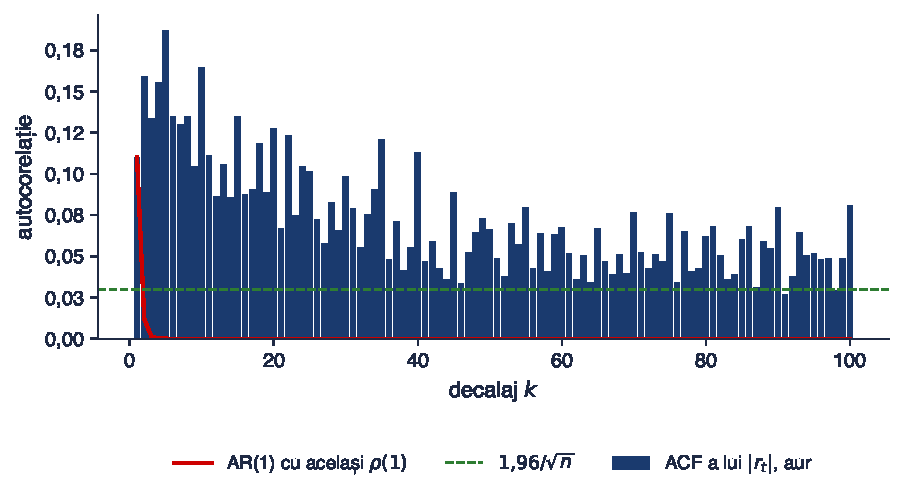
\includegraphics[width=0.64\textwidth]{practice_gold_absacf_ro.pdf}
\caption{Autocorelațiile lui $|r_t|$ pentru aur și ale unui AR(1) cu același $\rho(1)$.}\label{fig:goldacf}
\end{figure}
\begin{enumerate}
\item Calculați $\rho(10)$ și $\rho(100)$ pentru un AR(1) cu $\rho(1)=0{,}110$.
\item Estimați $d$ din panta legii de putere $\rho(k)\approx Ck^{2d-1}$, folosind decalajele 10 și 100.
\item Precizați un model potrivit pentru această volatilitate.
\end{enumerate}

% ===================================================================================================
\capitol{Capitolul 9. Învățare automată pentru serii de timp}

\pp{Semnul randamentului Bitcoin}
Două clasificatoare prognozează semnul randamentului Bitcoin de a doua zi, cu cinci decalaje și volatilitatea pe
20 de zile ca variabile explicative.
\softout{practice/out/p_btc_sign.txt}
\begin{enumerate}
\item Calculați statistica $z=(\hat a-a_0)/\sqrt{a_0(1-a_0)/n}$ pentru modelul random forest față de
reperul „întotdeauna în creștere”.
\item Explicați de ce reperul corect este clasa majoritară, nu acuratețea de 50\%.
\item Explicați de ce validarea încrucișată cu grupuri aleatoare ar supraestima acuratețea.
\end{enumerate}

\pp{Intervale conformale și funcția pinball: aurul}
Pentru randamentul zilnic al aurului se folosește prognoza punctuală 0, iar scorurile de conformitate sînt valorile
absolute ale erorilor. Cele 20 de scoruri de calibrare (ordonate) sînt: $0{,}13$; $0{,}14$; $0{,}32$; $0{,}53$; $0{,}63$;
$0{,}68$; $0{,}77$; $1{,}00$; $1{,}14$; $1{,}15$; $1{,}38$; $1{,}55$; $1{,}66$; $1{,}79$; $1{,}81$; $2{,}12$; $2{,}14$;
$2{,}90$; $3{,}01$; $4{,}05$. Randamentele din 14--18 septembrie 2026 sînt $-1{,}39$; $-0{,}12$; $-0{,}27$; $1{,}73$;
$0{,}77$.
\begin{enumerate}
\item Calculați intervalul conformal de 90\%, cu cuantila de ordinul $\lceil (n+1)(1-\alpha)\rceil$ a scorurilor.
\item Calculați ponderea randamentelor din 14--18 septembrie 2026 care cad în interval.
\item Calculați pierderea pinball medie, cu $\tau=0{,}05$, pentru cuantilele prognozate $q_A=-1{,}2$ și $q_B=-2{,}5$.
\end{enumerate}

% ===================================================================================================
\capitol{Capitolul 10. Modele în spațiul stărilor, filtrul Kalman și Markov switching}

\pp{Filtrul Kalman pentru rata șomajului din SUA}
Rata lunară a șomajului din SUA (2022--2025) a fost modelată cu un model local level, $y_t=\mu_t+\varepsilon_t$,
$\mu_{t+1}=\mu_t+\eta_t$. Valoarea din octombrie 2025 lipsește (nu a fost publicată).
\softout{practice/out/p_unrate_ll.txt}
În ianuarie 2026, rata șomajului a fost $4{,}3\%$.
\begin{enumerate}
\item Calculați raportul semnal--zgomot $q=\sigma^2_\eta/\sigma^2_\varepsilon$.
\item Calculați varianța predicției, cîștigul Kalman și nivelul filtrat pentru ianuarie 2026.
\item Descrieți pasul filtrului pentru luna lipsă (octombrie 2025).
\end{enumerate}

\pp{Regimuri de volatilitate: Nasdaq 100}
Randamentele săptămînale ale indicelui Nasdaq 100 (2015--2026) au fost modelate cu un model Markov switching cu două
regimuri.
\softout{practice/out/p_ndx_ms.txt}
\begin{enumerate}
\item Calculați durata medie a fiecărui regim, $1/(1-p_{ii})$, în săptămîni.
\item Calculați probabilitatea ergodică a regimului agitat.
\item Comparați probabilitatea ergodică cu ponderea observată a săptămînilor agitate.
\item Calculați volatilitatea anualizată (52 de săptămîni) a fiecărui regim.
\end{enumerate}

% ===================================================================================================
\clearpage
\capitol{Răspunsuri}
{\small
\begin{enumerate}[label=\textbf{\arabic*.},leftmargin=2.2em,itemsep=0.25ex]
\item (a) $\pm 1{,}96/\sqrt{100}=\pm 0{,}196$. (b) $Q(10)=88{,}13>18{,}31$: se respinge ipoteza de zgomot alb. (c) AR(1):
ACF scade treptat (8 din primele 10 autocorelații sînt în afara benzii), iar PACF este semnificativă doar la decalajul 1
($0{,}498$).
\item (a) $Q(5)=8{,}52$. (b) $8{,}52<11{,}07$: nu se respinge ipoteza că variațiile sînt necorelate (deși
$\hat\rho_1=-0{,}037$ este la limita benzii $\pm 0{,}036$). (c) Pentru un mers aleator, ACF de selecție rămîne aproape
de 1 pe multe decalaje; nivelul nu revine la o medie constantă, iar staționaritatea se obține prin diferențiere.
\item (a) $E(Y_t)=0$; $\mathrm{Var}(Y_t)=\sigma^4$. (b) Fiecare termen al produsului conține un $\varepsilon$ care
apare o singură dată, cu media 0. (c) $\mathrm{Cov}(Y_t^2,Y_{t-1}^2)=3\sigma^8-\sigma^8=2\sigma^8$;
$\mathrm{Var}(Y_t^2)=9\sigma^8-\sigma^8=8\sigma^8$; corelația este $0{,}25$: zgomot alb, dar nu independent.
\item (a) $\phi_1+\phi_2=0{,}702<1$; $\phi_2-\phi_1=-2{,}079<1$; $|\phi_2|=0{,}689<1$: staționar.
(b) $\phi_1^2+4\phi_2=-0{,}821<0$. (c) $\cos(2\pi/P)=0{,}838$; $P=10{,}9$ ani. (d) $\hat y_{2009}=13{,}69$.
\item (a) AIC: ARMA(2,0); BIC: ARMA(0,1). (b) Toate valorile $p$ sînt sub $0{,}05$: rămîne autocorelație în reziduuri
(cel mai puțin la AR(2), $p=0{,}034$); modelele sînt prea simple. (c) $0{,}184$; $0{,}130$. (d)
$\sqrt{1{,}015(1+0{,}202^2)}=1{,}028$.
\item (a) $\gamma(0)=\sigma^2(1+\theta^2)$, $\gamma(1)=\theta\sigma^2$, $\gamma(k)=0$ pentru $k\ge 2$.
(b) $0{,}4\theta^2-\theta+0{,}4=0$: $\theta=0{,}5$ sau $\theta=2$. (c) $\theta=0{,}5$, singura valoare inversabilă
($|\theta|<1$).
\item (a) $-0{,}407>-3{,}433$: nu se respinge rădăcina unitară. (b) $-14{,}04<-2{,}876$: se respinge. (c) $I(1)$.
(d) Nivelul are o tendință, deci constantă și trend; diferența fluctuează în jurul unei medii nenule, deci constantă.
\item (a) $z=-0{,}185$, $p=0{,}853$: $\theta$ nu este semnificativ. (b) Un mers aleator cu derivă este suficient. (c) $840{,}723$; $841{,}434$. (d) $4{,}667$; $6{,}561$. (e) $e^{8{,}40723}=4479{,}3$ USD pe uncie.
\item (a) ADF nu respinge rădăcina unitară ($p=0{,}610$), KPSS respinge staționaritatea ($0{,}260>0{,}146$): rădăcină
unitară. (b) ADF respinge ($p=0{,}001$), KPSS nu respinge ($0{,}203<0{,}463$): inflația este staționară.
(c) $\ln\mathrm{CPI}\sim I(1)$.
\item (a) $(1-L)(1-L^{12})y_t=(1-0{,}352L)(1-0{,}858L^{12})\varepsilon_t$. (b) Coeficientul lui $\varepsilon_{t-13}$ este $\theta\Theta=0{,}302$. (c) $Q(24)=19{,}42<33{,}92$ ($p=0{,}619$): reziduurile sînt zgomot alb. (d) $\rho(1)=-0{,}313$; $\rho(12)=-0{,}494$.
\item (a) $0{,}617$ (naivă sezonieră); $1{,}381$ (SARIMA). (b) $\mathrm{DM}=-2{,}04$. (c) $|-2{,}04|>1{,}96$: se respinge
acuratețea egală; metoda naivă sezonieră este mai bună. (d) Modelul subestimează puternic primăvara (aprilie: $1{,}256$
față de $1{,}716$; mai: $1{,}595$ față de $2{,}256$): estimat pe 2015--2024, cu anii pandemiei, nu surprinde nivelul de
după 2022, pe care metoda naivă sezonieră îl preia direct din 2024.
\item (a) Iulie: $-4{,}23\%$; august: $-4{,}38\%$. (b) Produsul telescopează: $(1-L)\sum_{j=0}^{11}L^j=1-L^{12}$.
(c) $(1-L^{12})s_t=s_t-s_{t-12}=0$.
\item (a) $\alpha+\beta=0{,}9815$. (b) $\bar\sigma^2=0{,}0364/0{,}0185=1{,}968$; $1{,}403\%$ pe zi; $22{,}27\%$ pe an. (c) $\ln 0{,}5/\ln 0{,}9815=37{,}1$ zile. (d) $6/1{,}468=4{,}09$. (e) Cozi groase; boltirea este finită pentru că $\nu>4$.
\item (a) $0{,}503+0{,}064\cdot 6{,}413^2+0{,}911\cdot 10{,}225=12{,}45$ ($\varepsilon_T=6{,}413$). (b) $\sigma=3{,}528$;
VaR 1\% $=2{,}326\cdot 3{,}528-0{,}083=8{,}12\%$. (c) $10\,000\,(1-e^{-0{,}0812})=780$ USD.
\item (a) $\mathrm{LR}=2(-6134{,}20+6203{,}10)=137{,}8>3{,}84$: se alege GJR-GARCH. (b) $1{,}744$ și $0{,}908$.
(c) $0{,}973$. (d) Doar șocurile negative cresc volatilitatea de a doua zi (efectul de levier).
\item (a) AIC: 6; BIC: 1; HQIC: 3. (b) $3(1+18)=57$ și $3(1+3)=12$. (c) $p=0{,}065$: nu se respinge la 5\%, se respinge
la 10\%. (d) $p=0{,}045$: creșterea PIB precedă în sens Granger rata dobînzii (reacția politicii monetare).
\item (a) Urma $0{,}279$, determinantul $-0{,}0173$; $\lambda_{1,2}=0{,}331$ și $-0{,}052$, în modul sub 1: VAR stabil.
(b) $\hat g=2{,}970$; $\widehat{\Delta i}=-0{,}030$. (c) $\mu=(3{,}091;\ -0{,}019)$.
\item (a) $R^2=0{,}690>\mathrm{DW}=0{,}038$: semnalul unei regresii false (regula Granger--Newbold). (b) $-2{,}56>-3{,}34$:
nu se respinge ipoteza nulă de absență a cointegrării. (c) Reziduurile provin dintr-o regresie estimată (OLS le minimizează varianța), deci
statistica este deplasată spre valori negative; sînt necesare valorile critice Engle--Granger.
\item (a) $26{,}25>15{,}49$ respinge $r=0$; $2{,}83<3{,}84$ nu respinge $r\le 1$: rangul 1. (b)
$\mathrm{GS10}=1{,}276+1{,}026\,\mathrm{TB3MS}$. (c) Dobînda pe 10 ani urmează dobînda pe 3 luni aproape unu la unu, plus o
primă de termen de circa $1{,}3$ puncte procentuale. (d) $1-0{,}0174-1{,}026\cdot 0{,}0236=0{,}958$; $16{,}3$ luni. (e) $z=-0{,}819$. (f) Corecțiile: $+0{,}014$ (GS10) și $-0{,}019$ (TB3MS) puncte procentuale pe lună.
\item (a) $[0{,}489;\ 0{,}779]$. (b) $z=1{,}81<1{,}96$: nu se respinge $d=0{,}5$. (c) Seria este la limita staționarității, cu memorie lungă și revenire la medie ($d<1$). (d) $-0{,}376\approx 0{,}634-1$. (e) $-0{,}630$;
$-0{,}117$; $-0{,}053$.
\item (a) $0{,}11^{10}=2{,}6\cdot 10^{-10}$; $0{,}11^{100}\approx 10^{-96}$. (b) Panta $\ln(0{,}081/0{,}164)/\ln 10=-0{,}306$;
$d=0{,}35$. (c) Un model cu memorie lungă pentru volatilitate: FIGARCH, HAR sau ARFIMA pentru volatilitatea realizată.
\item (a) $z=(0{,}495-0{,}504)/\sqrt{0{,}504\cdot 0{,}496/992}=-0{,}57$. (b) Proporția zilelor de creștere este peste
50\%; un model fără informație obține deja $50{,}4\%$. (c) Țintele și variabilele vecine se suprapun în timp (volatilitatea
pe 20 de zile); grupurile aleatoare pun în antrenare zile de după data testată (scurgere de informație).
\item (a) $\lceil 21\cdot 0{,}9\rceil=19$; $\hat q=3{,}01$; intervalul $[-3{,}01;\ 3{,}01]$. (b) $5/5$. (c) $L_A=0{,}105$;
$L_B=0{,}132$: cuantila $q_A$ are pierderea mai mică.
\item (a) $q=0{,}0059/0{,}0037=1{,}6$. (b) $P=0{,}0026+0{,}0059=0{,}0085$; $K=0{,}0085/(0{,}0085+0{,}0037)=0{,}697$;
$a=4{,}421+0{,}697(4{,}3-4{,}421)=4{,}337$. (c) Se omite actualizarea ($a_{t|t}=a_t$, $P_{t|t}=P_t$) și se face doar
predicția: varianța crește cu $\sigma^2_\eta$.
\item (a) $1/0{,}040=25{,}0$ săptămîni (calm); $1/0{,}062=16{,}1$ săptămîni (agitat). (b) $0{,}040/0{,}102=0{,}392$. (c) Valoare apropiată de ponderea observată, $0{,}376$. (d) $\sqrt{52\cdot 3{,}2}=12{,}9\%$; $\sqrt{52\cdot 14{,}335}=27{,}3\%$.
\end{enumerate}}
\end{document}
